\documentclass[12pt, twoside]{article}
\usepackage[letterpaper, margin=1in, headsep=0.2in]{geometry}
\setlength{\headheight}{0.6in}
%\usepackage[english]{babel}
\usepackage[utf8]{inputenc}
\usepackage{microtype}
\usepackage{amsmath}
\usepackage{amssymb}
%\usepackage{amsfonts}
\usepackage{siunitx} %units in math. eg 20\milli\meter
\usepackage{yhmath} % for arcs, overparenth command
\usepackage{tikz} %graphics
\usetikzlibrary{quotes, angles}
\usepackage{graphicx} %consider setting \graphicspath{{images/}}
\usepackage{parskip} %no paragraph indent
\usepackage{enumitem}
\usepackage{multicol}
\usepackage{venndiagram}

\usepackage{fancyhdr}
\pagestyle{fancy}
\fancyhf{}
\renewcommand{\headrulewidth}{0pt} % disable the underline of the header
\raggedbottom
\hfuzz=2mm %suppresses overfull box warnings

\usepackage{hyperref}

\fancyhead[LE]{\thepage}
\fancyhead[RO]{\thepage \\ Name: \hspace{4cm} \,\\}
\fancyhead[LO]{BECA / Dr. Huson / Geometry\\*  Unit 12: Trigonometry \\* 21 March 2023}

\begin{document}

\subsubsection*{12.7 Extension: Regents trigonometry problems \hfill HSG.SRT.C.8}
\begin{enumerate}
  \subsubsection*{Start by sketching the situation for each problem}

\item A 12-foot ladder leans against a building and reaches a window 10 feet above ground. What is the measure of the angle, to the \emph{nearest degree}, that the ladder forms with the ground? \vspace{5cm}

\item A support wire reaches from the top of a pole to a clamp on the ground. The pole is perpendicular to the level ground and the clamp is 10 feet from the base of the pole. The support wire makes a $68^\circ$ angle with the ground. Find the length of the support wire to the \emph{nearest foot}. \vspace{6cm}

\item In right triangle $ABC$, hypotenuse $\overline{AB}$ has a length of 26 cm, and side $\overline{BC}$ has a length of 17.6 cm. What is the measure of angle $B$, to the \emph{nearest degree}?

\newpage
\item Regents January 2019\\
 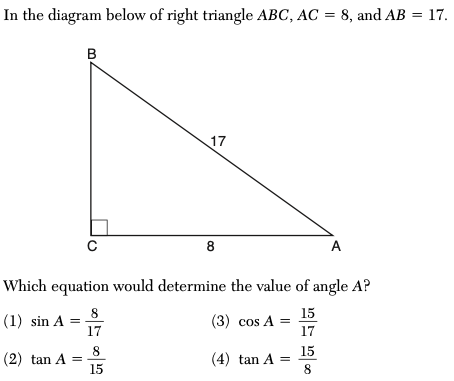
\includegraphics[scale=0.65]{../graphics/Pyth+trig_17_Jan2019.png}

\subsubsection*{Sine and cosine values of complementary angles \hfill HSG.SRT.C.7}
\item Regents June 2019\\
 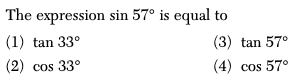
\includegraphics[scale=0.65]{../graphics/sine-cos-9_Jun2019.png}

\item Regents Jan 2019 \\
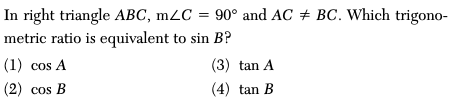
\includegraphics[scale=0.65]{../graphics/sine-cos-9_Jan2019.png}

\item If $\sin(2x+7)^\circ = \cos(4x-7)^\circ$, what is the value of $x$? \hfill Regents August 2018
\vspace{1cm}

\item In a right triangle, the acute angles have the relationship $\sin(2x + 4) =\cos (46)$. \\[0.25cm]
What is the value of $x$? \hfill Regents June 2018

\end{enumerate}
\end{document}
  